\documentclass[../main.tex]{subfiles}
\begin{document}
The chapter report the development process for the software dashboard, starting from explaining the requirements behind the needs of a software dashboard and how this helps developer in the process of generating software for motor \gls{ECUM}s. The chapter report the path towards the construction of the dashboard following the flow that the data has inside the pipeline that brings always updating data to the dashboard itself. The first part discuss the software structure at \gls{BMW} and the data related to it, then the code that generated this data is reported, keeping an eye on the data side of this. Concluding the chapter report the pipeline implementations and the details related to the dashboard itself.
\section{Dashboard objective definition}
As already introduced in the Thesis abstract the development of \gls{ECU} software is complex process. As each complex process composed by multiple step there is always the requirement of tracking results, quality and completeness of each step. In order to do that a high load of data is generated during each step in order to have a feedback on the status of execution.\\
In the development of \gls{ECU} software most of the steps to create software are divided on multiple departments and then additionally divided between the single member of a team. Each of the person responsible for a single task keep track of the data of that single task. Most of the time only single person know where the data for the single task lay and also how to read those data. This can create problem especially when people outside the task require information for it. They always need to refer to the person in charge. A centralized view on the process is missing, as also a centralize storing repository for the data. \\
The idea to create a database to store data in a readable form and the to create graphical visualization, namely dashboard of the data, is the idea that want to full fill the previous raised problem.\\
Via a dashboard with updated data different developers in different teams can simultaneously surf thought the data and get real time information on the status of the process, thus increasing the feedback on every task and therefor the output result.
\subsection{Data pipeline concept}
The concept of having data flowing from the source that generates the data all the way to the dashboard can be summarized un der the name pipeline. This gives an idea of the basic concept that the flow of data need to have. The data need to be always updated, the flow need to be controlled by some mechanism that take the updating data and push it to the different steps of the pipe all the way to the dashboard itself. Three main steps cna be identified in the pipeline:

\tikzstyle{block} = [draw, rectangle, text width=3.5cm, text centered, minimum height=1.2cm, node distance=6cm]
\begin{figure}[h]
  \centering
\begin{tikzpicture}[scale=0.85,transform shape]
    \node [block, name=text1] {Data Source};
    \node [block, right of=text1] (text2) {Data Storage};
    \node [block, right of=text2] (text3) {Data Visulization};

    \draw [->] (text1) -- (text2);
    \draw [->] (text2) -- node {} (text3);

\end{tikzpicture}
  \caption{General pipeline structure}
  \label{pipelinestructure}
\end{figure}

\begin{itemize}
    \item Data source, in this case the data source is the EA-build software. As reported in Section \ref{sec:EA-buildsection} the software is responsible for the compilation of the code and therefor for the generation of the data. 
    \item Data storage, the data generate in the first process is stored in a relational database, namely EA-dashboard. This database is the middleman between the data source and the dashboard. The database receives information from the data source, stores the information under the form of tables and deliver data to the dashboard.
    \item Data visualization, the data stored in the database gets queried and reorganized. Visualization are created in a interactive manner in a dashboard available for the whole team.
\end{itemize}
\begin{figure}[h]
    \centering
    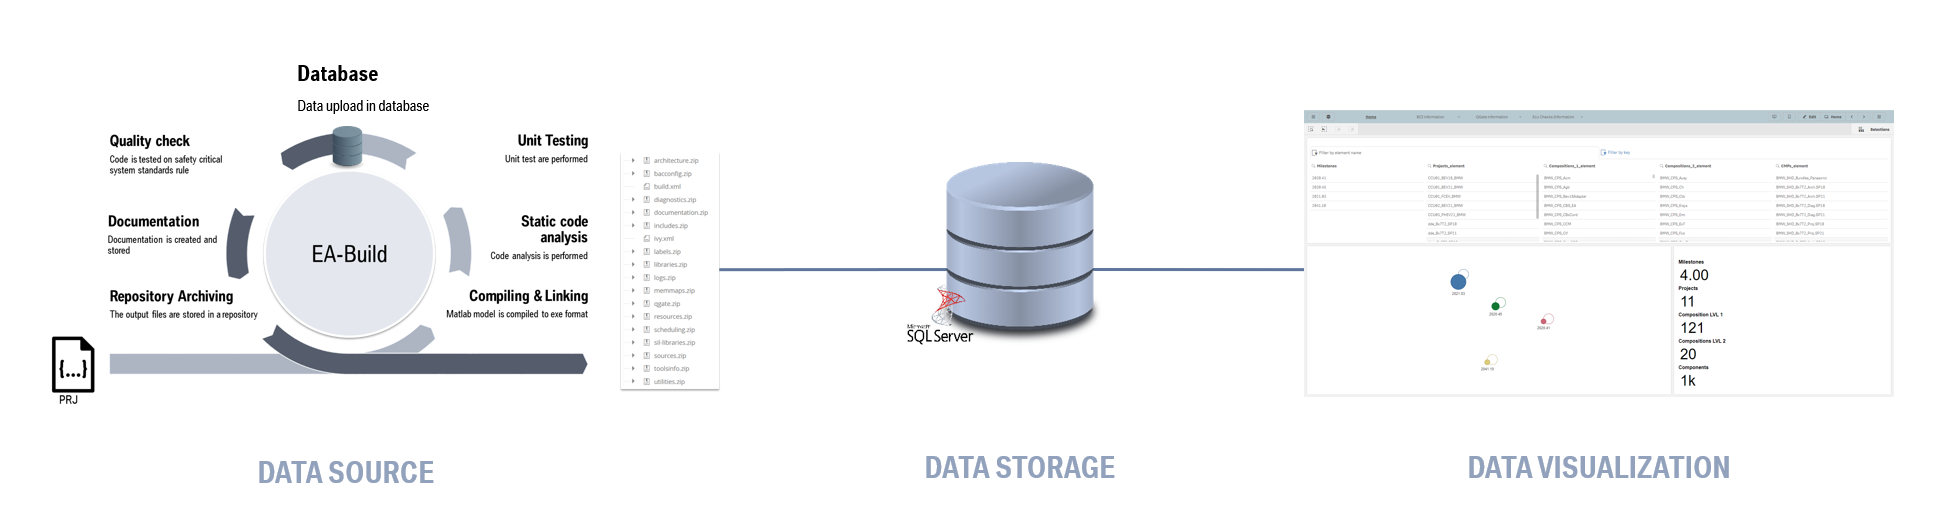
\includegraphics[width=\linewidth]{images_folder/pipeline_1.png}
    \caption{Pipeline structure}
    \label{fig:pipeline1}
\end{figure}
\section{Data Source}
The first part of the chapter introduce how the data is generated and what is the data related to software structure. Therefore during the section the software structure for \gls{ECU} is given and the data with an example of some batch data already integrated in the pipeline.
\subsection{Software structure for ECU}
In order to access and structure data there is the need of having a backbone structure, at which all the data can be related and can also be used to easily surf thought the data to search for relevant information. In this regard the software structure for \gls{ECU}s comes really in hand.\\ 
Software for \gls{ECU} is not developed as a single package. Software in packages for motor functional areas, each package namely compositions. A composition can refer to the full ignition system control. Under this composition other can be found all the way to the single software components that control the flow of fuel.\\
In the structure the sum of different composition define a project. A project refer to a different engine. One level up from composition we find the milestones, those refer to the baseline at which the software is consider, as explained in the chapter over Software Management Configuration. In general a Milestone follow the Scrum cycles, but there can be differences. \\
\begin{figure}
    \centering
    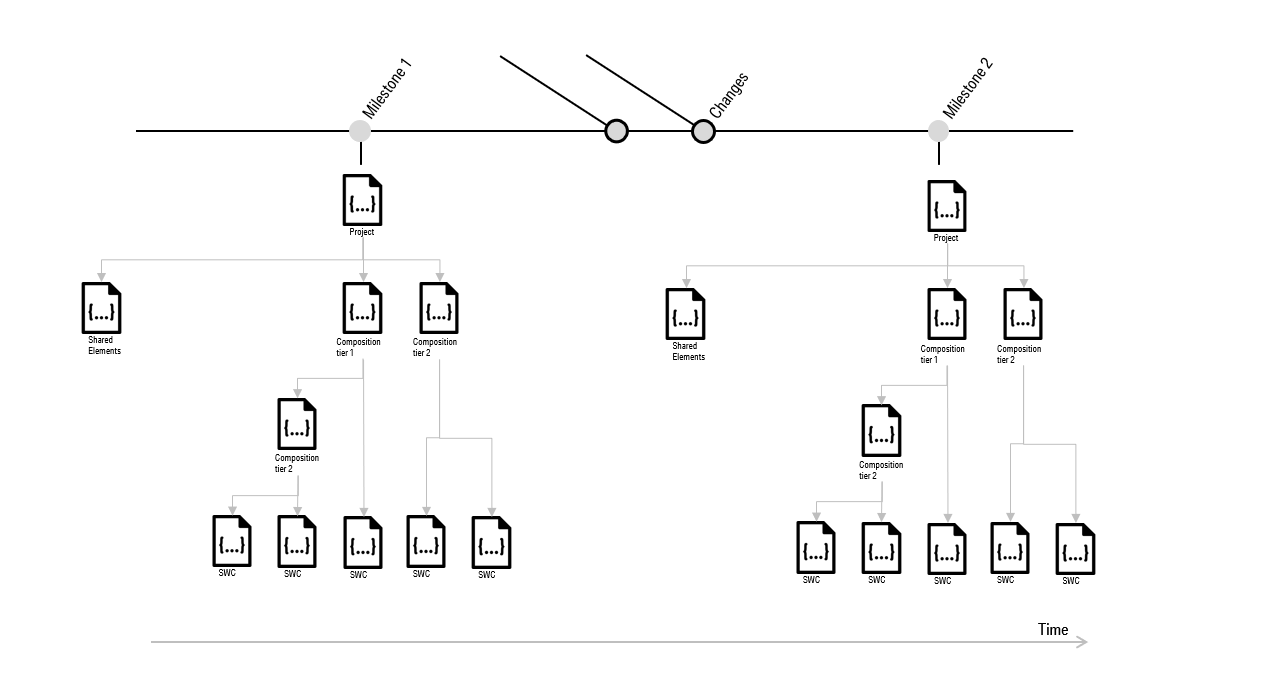
\includegraphics[width=\linewidth]{images_folder/softwarestrucutre.png}
    \caption{Software structure}
    \label{fig:SWsTR}
\end{figure}
\section{Hierarchical structure and primary key decisions}
\section{MVP definition}
\subsection{Double layering the primary key - Double layer of abstraction introduced}
\section{Database integration}
\section{Piepline steps definition}
\section{Instantiation of a Jenkins job}
\subsection{Propsor information}
\subsection{BCI information}
\cleardoublepage
\end{document}